% \iffalse
\let\negmedspace\undefined
\let\negthickspace\undefined
\documentclass[beamer]{IEEEtran}
\usepackage{cite}
\usepackage{amsmath,amssymb,amsfonts,amsthm}
\usepackage{algorithmic}
\usepackage{graphicx}
\usepackage{textcomp}
\usepackage{xcolor}
\usepackage{txfonts}
\usepackage{listings}
\usepackage{enumitem}
\usepackage{mathtools}
\usepackage{gensymb}
\usepackage{comment}
\usepackage[breaklinks=true]{hyperref}
\usepackage{tkz-euclide} 
\usepackage{listings}
\usepackage{gvv}                                        
\def\inputGnumericTable{}                                 
\usepackage[latin1]{inputenc}                                
\usepackage{color}                                            
\usepackage{array}                                            
\usepackage{longtable}                                       
\usepackage{calc}                                             
\usepackage{multirow}                                         
\usepackage{hhline}                                           
\usepackage{ifthen}                                           
\usepackage{lscape}
\usepackage[export]{adjustbox}

\newtheorem{theorem}{Theorem}[section]
\newtheorem{problem}{Problem}
\newtheorem{proposition}{Proposition}[section]
\newtheorem{lemma}{Lemma}[section]
\newtheorem{corollary}[theorem]{Corollary}
\newtheorem{example}{Example}[section]
\newtheorem{definition}[problem]{Definition}
\newcommand{\BEQA}{\begin{eqnarray}}
\newcommand{\EEQA}{\end{eqnarray}}
\newcommand{\define}{\stackrel{\triangle}{=}}
\theoremstyle{remark}
\newtheorem{rem}{Remark}
\begin{document}
\parindent 0px
\bibliographystyle{IEEEtran}

\title{Assignment\\[1ex]10.5.4-2}
\author{ee23btech11215 - Penmetsa Srikar Varma$^{}$% <-this % stops a space
}
\maketitle
\newpage
\bigskip

\renewcommand{\thefigure}{\theenumi}
\renewcommand{\thetable}{\theenumi}
\section*{Question:}
Q2) The sum of the third and the seventh terms of AP is 6 and their product is 8. Find the sum of first sixteen terms of the AP\\
\section*{Solution:}
{
\centering
Table of Parameters\\
}
\begin{table}[h]
    \centering
    \begin{tabular}{|c|c|}
    \hline
     Input Variables & Input Condition \\
\hline
     x\brak{2}+x\brak{6}& 6 \\
\hline
     x\brak{2}.x\brak{6} & 8 \\
\hline
     $x_i$\brak{n} &  general term of $\text{i}^\text{th}$ AP sequence\\
\hline
     $y_i$\brak{n} &  sum of first n terms of $\text{i}^\text{th}$ AP sequence\\
\hline
     $x_i$\brak{0} & first term of $\text{i}^\text{th}$ AP sequence\\
\hline
     $d_i$ & common difference of $\text{i}^\text{th}$ AP sequence\\
\hline
     $x_i\brak{n}\system{Z}X_i\brak{z}$ & $z$-transform of $x_i\brak{n}$ \\
\hline
     $y_i\brak{n}\system{Z}Y_i\brak{z}$ & $z$-transform of $y_i\brak{n}$ \\
\hline
    \end{tabular}

    \label{tab:my_label}
\end{table}

Then general term x\brak{n} of arithmetic progression is given by:
\begin{equation}
\label{q1}
x\brak{n}=x\brak{0}+n.d
\end{equation}
Then from \brak{\ref{q1}}:
\begin{equation}
\label{q2}
x\brak{2} = x\brak{0}+2.d
\end{equation}
\begin{equation}
\label{q3}
x\brak{6}=x\brak{0}+6.d
\end{equation} 
Then from table of parameters,
\begin{align}
\label{q6}
    x\brak{2}=6-x\brak{6}
\end{align}
From \brak{\ref{q6}}
$$x\brak{2}.x\brak{6}=8$$
$$x\brak{6}.\brak{6-x\brak{6}}=8$$
\begin{align}
\label{q7}
    x\brak{6}=2\ or\ 4
\end{align}
Then from $\brak{\ref{q6}}$ and $\brak{\ref{q7}}$
\begin{align}
\label{q8}
    x\brak{2}=4\ or\ 2
\end{align}
from $\brak{\ref{q2}}$,$\brak{\ref{q3}}$ and $\brak{\ref{q7}}$,$\brak{\ref{q8}}$\\
for x$\brak{2}$ = 2 and x$\brak{6}$ = 4
\begin{align}
x\brak{0}=1,\ d=\frac{1}{2}
\end{align}

for x$\brak{2}$ = 4 and x$\brak{6}$ = 2
\begin{align}
x\brak{0}=5,\ d=-\frac{1}{2}
\end{align}

We know that the sum of first n terms of arithmetic progression is given by:
\begin{equation}
\label{q9}
S\brak{n}= \frac{n}{2}\brak{2.x\brak{0}+\brak{n-1}.d}
\end{equation}
Then from \brak{\ref{q9}} let sum of first 16 terms of arithmetic progression be $S_{16}$:
\begin{equation}
\label{q10}
S\brak{16}= \frac{16}{2}\brak{2.x\brak{0}+15d}
\end{equation}
Hence from \brak{\ref{q10}},
for $x\brak{0}$=1,d=$\frac{1}{2}$
\begin{align}
\label{11}
S_1\brak{16}=76
\end{align}
or from \brak{\ref{q10}},
for $x\brak{0}$=5,d=-$\frac{1}{2}$
\begin{align}
\label{12}
S_2\brak{16}=20
\end{align}
The general term of AP x\brak{n} and sum of first n terms of AP S\brak{n} are given by:
\begin{align}
x_1\brak{n}=\frac{n+2}{2}\quad and\quad S_1\brak{n}=\frac{n.\brak{n+3}}{4}
\end{align}
\begin{align}
x_2\brak{n}=\frac{10-n}{2}\quad and\quad S_2\brak{n}=\frac{n.\brak{21-n}}{4}
\end{align}

\begin{figure}[h]
    \centering
    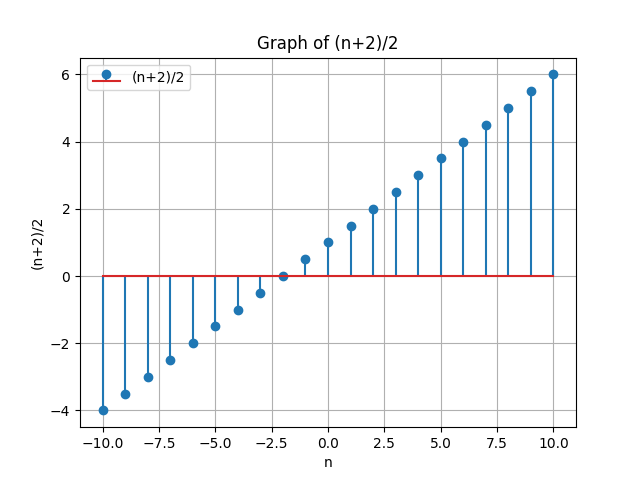
\includegraphics[scale=0.60]{py_3.png}
    \label{fig:enter-label}
    \caption*{Graph of $\frac{n+2}{2}$}
\end{figure}

\begin{figure}[h]
    \centering
    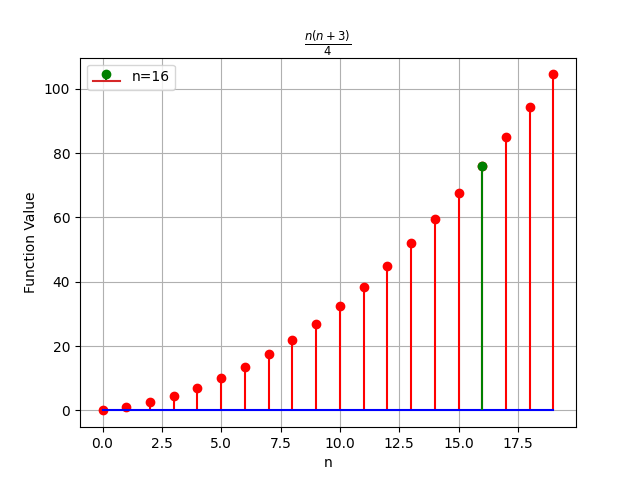
\includegraphics[scale=0.60]{py_4.png}
    \label{fig:enter-label}
    \caption*{Graph of $\frac{n\brak{n+3}}{4}$}
\end{figure}

\begin{figure}[h]
    \centering
    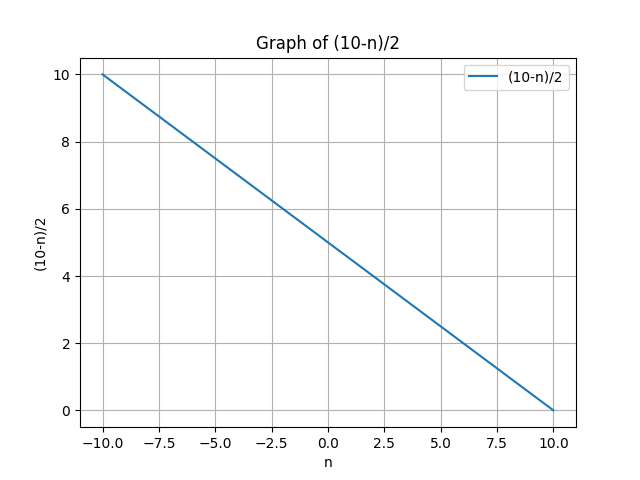
\includegraphics[scale=0.60]{py_5.png}
    \label{fig:enter-label}
    \caption*{Graph of $\frac{10-n}{2}$}
\end{figure}

\begin{figure}[h]
    \centering
    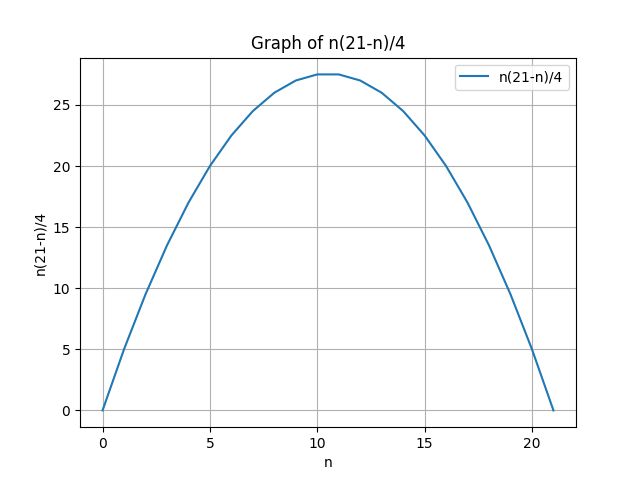
\includegraphics[scale=0.60]{py_6.png}
    \label{fig:enter-label}
    \caption*{Graph of $\frac{n\brak{21-n}}{4}$}
\end{figure}
We know that Z-Transform of x\brak{n} is given by:
\begin{align}
\label{q11}
    X\brak{z}=\sum_{k=-\infty}^{\infty} x\brak{k}.z^{-k}
\end{align}
where, we assume that x\brak{k}=0   for \brak{k<0}\\
Then, \brak{\ref{q11}} modifiy as follows:
\begin{align}
\label{q12}
    X_1\brak{z}=\sum_{k=0}^{\infty} x_1\brak{k}.z^{-k}
\end{align}
\begin{align}X_1\brak{z}=\sum_{k=0}^{\infty} \brak{\frac{k+2}{2}}.z^{-k}\end{align}
\begin{align}
    \label{q13}
    X_1\brak{z}=\frac{1}{2}\brak{\sum_{k=0}^{\infty}k.z^{-k}}+\sum_{k=0}^{\infty}z^{-k}
\end{align}
\begin{align}
    \label{q13}
    X_1\brak{z}=\frac{1}{2}\brak{\frac{z^{-1}}{\brak{1-z^{-1}}^2}}+\frac{1}{1-z^{-1}}
\end{align}
So,
\begin{align} X_1\brak{Z}=\frac{2-z^{-1}}{2.\brak{1-z^{-1}}^2}\quad for\ |z^{-1}|<1\end{align}
or,
\begin{align}
X_1\brak{Z}\ is\ not\ defined\qquad for\ |z^{-1}|>1 
\end{align}
From \brak{\ref{q12}},
\begin{align}
    X_2\brak{z}=\sum_{k=0}^{\infty} x_2\brak{k}.z^{-k}
\end{align}
\begin{align}X_2\brak{Z}=\sum_{k=0}^{\infty} \brak{\frac{10-k}{2}}.z^{-k}\end{align}
\begin{align}X_2\brak{Z}=5.\brak{\sum_{k=0}^{\infty}z^{-k}}-\frac{1}{2}\brak{\sum_{k=0}^{\infty}k.z^{-k}}\end{align}
\begin{align}X_2\brak{Z}=5.\brak{\frac{1}{1-z^{-1}}}-\frac{1}{2}\brak{\frac{z^{-1}}{\brak{1-z^{-1}}^2}}\end{align}
So,
\begin{align}X_2\brak{Z}=\frac{11.\brak{1-z^{-1}}-1}{2.\brak{1-z^{-1}}^2}\quad for\ |z^{-1}|<1\end{align}
or,
\begin{align}X_2\brak{Z}\ is\ not\ defined\quad for\qquad |z^{-1}|>1\end{align}
\begin{figure}[h]
    \centering
    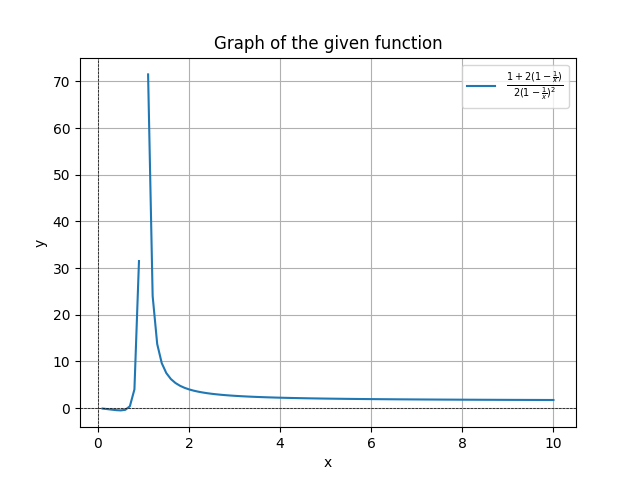
\includegraphics[scale=0.52]{py_31.png}
    \label{fig:enter-label}
    \caption*{Graph of $\frac{2-z^{-1}}{2.\brak{1-z^{-1}}^2}$}
\end{figure}
\begin{figure}[h]
    \centering
    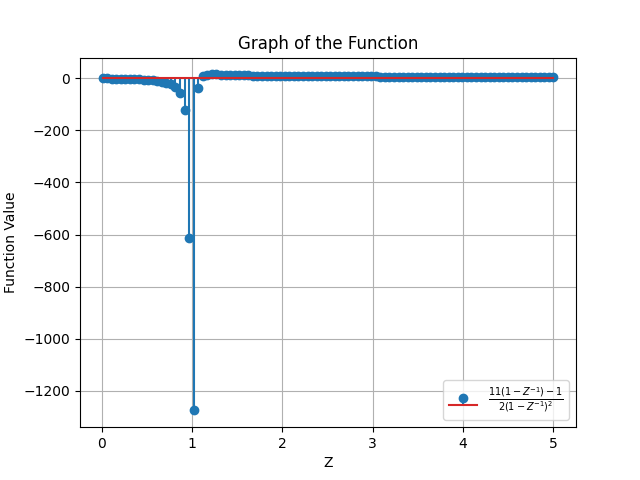
\includegraphics[scale=0.52]{py_32.png}
    \label{fig:enter-label}
    \caption*{Graph of $\frac{11.\brak{1-z^{-1}}-1}{2.\brak{1-z^{-1}}^2}$}
\end{figure}

Let, $\mathcal{Z}$ tranform of s(n) be S(Z):\\
from \brak{\ref{q11}}:
$$S\brak{Z}=\sum_{k=-\infty}^{\infty}s(k)\ z^{-k}=\sum_{k=0}^{\infty}s(k)\ z^{-k}\quad \brak{s\brak{k}=0\ for\ k<0}$$
from \brak{\ref{q9}}
\begin{align}
S\brak{Z}=\sum_{k=-\infty}^{\infty}\left(\brak{x\brak{0}-\frac{d}{2}}k+\frac{d}{2}\ k^2\right).z^{-k}
\end{align}

\begin{align}
\label{q17}
    S\brak{Z}=\brak{x\brak{0}-\frac{d}{2}}\left(\sum_{k=0}^{\infty}k.Z^{-k}\right)+\frac{d}{2}.\left(\sum_{k=0}^{\infty}k^2.Z^{-k}\right)
\end{align}

\begin{align}
    S\brak{Z}=\brak{x\brak{0}-\frac{d}{2}}\left(\frac{z^{-1}}{\brak{1-z^{-1}}^2}\right)+\frac{d}{2}.\left(\frac{z^{-1}\brak{1+z^{-1}}}{\brak{1-z^{-1}}^3}\right)
\end{align}

\begin{align}
s\brak{Z}=x\brak{0}\left(\frac{z^{-1}}{\brak{1-z^{-1}}^2}\right)+d\left(\frac{z^{-2}}{\brak{1-z^{-1}}^3}\right)
\end{align}

\begin{align}
\label{w1}
s\brak{Z}=x\brak{0}\brak{\frac{z}{\brak{z-1}^2}}+d\brak{\frac{z}{\brak{z-1}^3}}
\end{align}

for x\brak{0}=1 and $d=\frac{1}{2}$

\begin{align}S_1\brak{Z}=\frac{z^{-1}\brak{1-\frac{1}{2}z^{-1}}}{\brak{1-z^{-1}}^3}\end{align}

\begin{figure}[h]
    \centering
    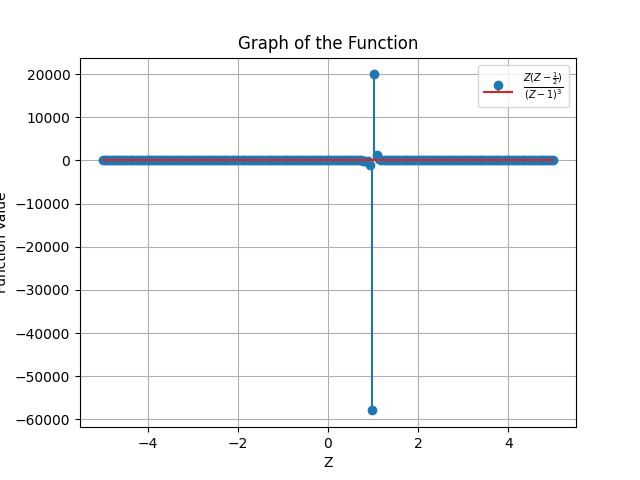
\includegraphics[scale=0.52]{py_33.png}
    \label{fig:enter-label}
    \caption*{Graph of $\frac{z^{-1}\brak{1-\frac{1}{2}z^{-1}}}{\brak{1-z^{-1}}^3}$}
\end{figure}

for x\brak{0}=5 and $d=-\frac{1}{2}$

\begin{align}S_2\brak{Z}=\frac{z^{-1}\brak{5-\frac{11}{2}z^{-1}}}{\brak{1-z^{-1}}^3}\end{align}

\begin{figure}[h]
    \centering
    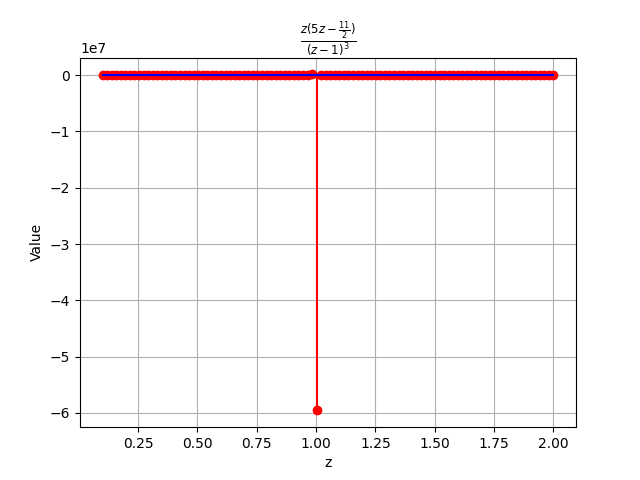
\includegraphics[scale=0.52]{py_34.png}
    \label{fig:enter-label}
    \caption*{Graph of $\frac{z^{-1}\brak{5-\frac{11}{2}z^{-1}}}{\brak{1-z^{-1}}^3}$}
\end{figure}

We know that Inverse $\mathcal{Z}$ - transform of $S\brak{z}$ say $s\brak{n}$, by counter integral method is given by:

\begin{align}
s\brak{n}=\oint_C S(z)\ z^{n-1}\, dz
\end{align}

from \brak{\ref{w1}},

\begin{align}
    s\brak{n}=x\brak{0}\oint_C \brak{\frac{z}{\brak{z-1}^2}dz} + d\brak{\oint_C  \frac{z}{\brak{z-1}^3} \, dz}
\end{align}

From residue theorem for similar residues:
\begin{align}
    s\brak{n}=x\brak{0}\left|\frac{1}{1!}\frac{d}{dz}\brak{z^n}\right|_{z=1} + d\left|\frac{1}{2!}\frac{d^2}{dz^2}\brak{z^n}\right|_{z=1}
\end{align}

\begin{align}
    s\brak{n}=n.x\brak{0} + n\brak{n-1}\frac{d}{2}
\end{align}
\begin{align}
\label{39}
    s_1\brak{n}=\frac{n\brak{n+3}}{4},s_1\brak{16}=76
\end{align}
and,
\begin{align}
\label{40}
    s_2\brak{n}=\frac{n\brak{21-n}}{4},s_2\brak{16}=20
\end{align}

we can observe that \brak{\ref{11}} and \brak{\ref{39}},\brak{\ref{12}} and \brak{\ref{40}} are the same results
\end{document}
